\documentclass[preview]{standalone}
\usepackage{tkz-graph}
\begin{document}

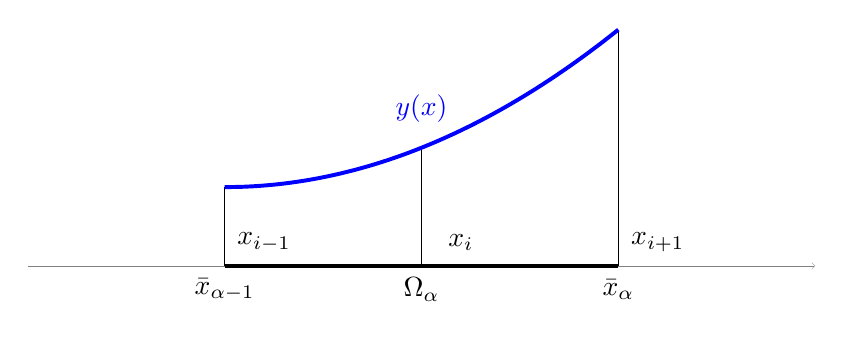
\begin{tikzpicture}
\draw[->,ultra  thin,color=gray] (-2.5,0) -- (7.5, 0);
\draw[line width=0.1mm, color=black] (0,0) -- (0, 1);
\draw[line width=0.1mm, color=black] (2.5,0) -- (2.5, 1.5);
\draw[line width=0.1mm, color=black] (5,0) -- (5, 3);
\draw[line width=0.5mm, color=black] (0,0) -- (5, 0);
\draw[blue, line width = 0.5mm]   plot[smooth,domain=0:5] (\x, {1+0.08*(\x)^2});
\draw (0, -0.3) node {$\bar{x}_{\alpha-1}$};
\draw (5, -0.3) node {$\bar{x}_{\alpha}$};
\draw (2.5, -0.3) node {$\Omega_{\alpha}$};
\draw (0.5, 0.3) node {$x_{i-1}$};
\draw (3, 0.3) node {$x_{i}$};
\draw (5.5, 0.3) node {$x_{i+1}$};
\draw[color=blue] (2.5, 2) node {$y(x)$};
\end{tikzpicture}

\end{document}



После: convert pdf to png
https://convertio.co/pdf-png/



 






